\chapter[Data]{Data}
\label{ch:data}
The following chapter introduce the different types of data analyzed in this work. Synthetic data are generated an analyzed, for better control of behavior and result verification of the ACER and POT MCMC method before the methods are used for a variety of commodity times series.
\section{Synthetic Data}
Two synthetic data series are generated. Both attempts to test the methods on different aspects which are important for real life commodity analysis. The first is the thick tail Pareto distribution, since commodity data are fat tail distributed, as was concluded by \cite{fattail}.  The Pareto distribution can generate i.i.d. data which are easy to control and where exact analytic inference can be achieved. 

The second, numerically generates a time series with approximately the same distribution characteristics as the return of crude oil commodity data. Since it is a numeric method, the data can be generated as large as desired, and much larger than is practical achievable in real life. This makes test result and verification much more accurate than limited real life data.
\subsection{Pareto Distribution}
The Pareto distribution has the following cumulative distribution function
\begin{equation}
\label{eq:paretocdf}
\Pr(X<x)=
\begin{cases}
1-\frac{1}{x^\beta} & \quad x>1\\
0 & x<1\\
\end{cases}
\end{equation}
where $\beta$ is a shape parameter. A cumulative distribution function is said to have fat tail if \\$\Pr(X>x)\sim x^{-\beta}$, as $x \to \infty$,  for $\beta > 0$. By the definition, the Pareto distribution clearly has a fat tail.
Using the probability integral transform approach, a data point $x_i$ is generated by
\begin{equation}
x_i=\frac{1}{u_i^{1/\beta}},
\end{equation}
where $u_i \sim UNIF(0,1)$.

A practical data size could come from having a daily return each day for 25 years. Without considering leap year, roll-over returns, and weekend, that corresponds in a 25 times 365 data series. Multiple data series with this size was generated using $1<\beta<5$.
\begin{figure}
  \centering
    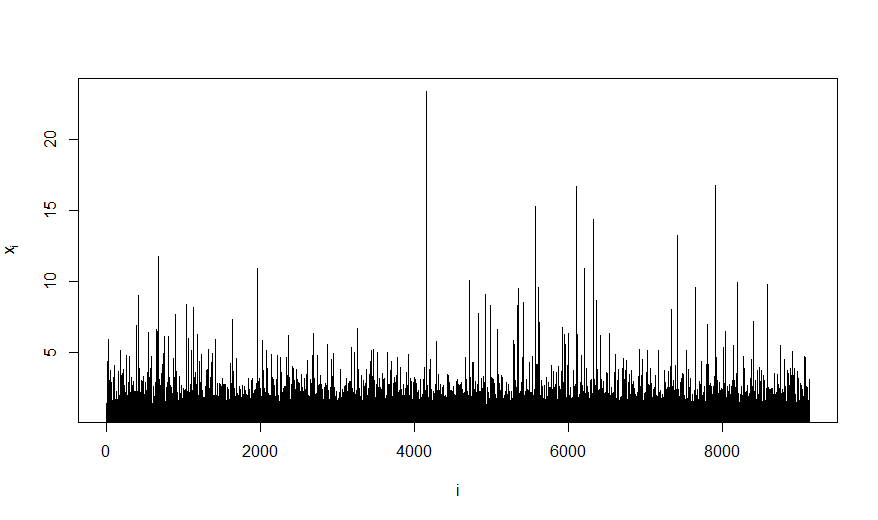
\includegraphics[width=1\textwidth]{fig/paretoreala.png}
  \caption{Generated Pareto distributed points with 9125 realization and $\beta=3$. The $i$ axis represent time in days, while $x_i$ is the realized data point for that day.}
  \label{fig:paretodata}
\end{figure}
Figure \ref{fig:paretodata} show a generated Pareto distributed time series for $\beta=3$, where the realizations range from $1.000$ to $23.384$.

\subsection{Generated Commodity Data}
As the Pareto distribution above generated i.i.d. data points, it seems logical to simulate dependent and homoscedastic data to reveal any performance difference of the methods. This work focus on the ACER and POT MCMC methods ability to capture the tail effect of commodity data, hence the ability to generating data with close to the same behaviors as real life commodity is desired. 

It was suggested by \cite{aparch} that The $\text{AR}(3)$-$\text{APARCH}(1,1)$, with skewed student $t$ distribution as error term, was a good approximation for the commodity time series. Starting with the suggested model, the AIC, BIC and log likelihood ratio test was applied to the neighboring models, for model selection. Using the observed crude oil daily return described below in chapter \ref{ch:comdata}, the parameters for $\text{AR}(3)$-$\text{APARCH}(1,1)$, and neighboring models, can be estimated. The AIC, BIC and the log likelihood ratio test favors a higher AR dependency, while MA and additional APARCH parameters does not improve the model significantly. As the test show sign of a high AR dependency, selecting the model comes down to accuracy against computational intensity. The $\text{AR}(4)$- $\text{APARCH}(1,1)$ is concluded as a reasonable good model with lower AIC and BIC than its neighbors, and the log likelihood ratio test showing significantly improvements from all subsets, while $\text{AR}(5)$- $\text{APARCH}(1,1)$ does not significantly improve the model. The estimated parameters of $\text{AR}(4)$- $\text{APARCH}(1,1)$ with $\mu=6.34\cdot 10^{-4}$ is presented in table \ref{table:ar4aparch11para}.
\textcolor{red}{SKRIV LITT OM TROR MODEL AR(5) ER EN DEL BEDRE ENN AR(4)}


\begin{table}[h]
\centering
\begin{tabular}{ l c c}
    & Estimate & p-value\\
  \hline
  $\phi_1$ & $-2.586\cdot 10^{-2}$ & $0.0833$ \\
  $\phi_2$ & $-4.339\cdot 10^{-2}$ & $3.66\cdot 10^{-3}$ \\
  $\phi_3$ & $-1.699\cdot 10^{-2}$ & $0.236$ \\
  $\phi_4$ & $-4.682\cdot 10^{-3}$ & $0.751$ \\
  $\omega$ & $9.869\cdot 10^{-5}$ & $2.43\cdot 10^{-3}$\\
  $\alpha_1$& $5.557\cdot 10^{-2}$ & $<2\cdot 10^{-16}$\\
  $\gamma_1$& $2.215\cdot 10^{-1}$ & $356 \cdot 10^{-3}$ \\
  $\beta_1$ & $9.498\cdot 10^{-1}$ & $<2\cdot 10^{-16}$\\
  $\delta$ & $1.123$ & $1.71 \cdot 10^{-7}$\\
  $\xi$ & $9.682 \cdot 10^{-1}$ & $<2\cdot 10^{-16}$\\
  $\nu$ & $7.333$ & $<2\cdot 10^{-16}$\\
\end{tabular}
\caption{}
\label{table:ar4aparch11para}
\end{table}



\cite{aparch} %aparch VaR
\section{Commodity Data}
\label{ch:comdata}
Adjusted for the roll-over returns. (simply done by deleting the return at the roll-over date).(roll-over, en kontrakt til neste eks sommer til hoest, kan gi ekstreme returns som gir  forvrengende resultater).
blabla